\section{模型的构建与实现}\label{sec:3}

此次实验为了探究预训练编码模型BERT对于对情感识别领域中的对话情感识别的作用。本章首先介绍此次实验所用到的数据集,然后介绍主要模型的结构,最后给出实验结果和实验的各种细节。

\subsubsection{数据集与预处理过程}

本次实验的数据集来自DailyDialog\cite{dailydialog},这是一个用于对话系统和情感识别的常用数据集。数据集中的对话是来自于日常生活中真实的对话,包括了多样的情感和语境。相比于来源于Twitter和微博的数据集,DailyDialog数据集中的数据来自于英语学习者相关的网站,并且使用了一个开源的英文自动纠错程序来消除了简单的英语单词拼写错误问题,使其主题相对集中,语法相对规范。一个数据实例如表\ref{table:DailyDialog}所示。

\begin{table}[!ht]
	\caption{DailyDialog数据集数据展示}
	\label{table:DailyDialog}
	\centering
	\begin{tabular*}{\textwidth}{c@{\extracolsep{\fill}}cc}
		\toprule
		\textbf{对话句子} & \textbf{情绪} & \textbf{行动} \\ \midrule
		So Dick , how about getting some coffee for tonight ? & 快乐 & 指令 \\ 
		Coffee ? I don ’ t honestly like that kind of stuff . & 厌恶 & 承诺 \\ 
		Come on , you can at least try a little , besides your cigarette . & 没有情绪 & 指令 \\ 
		What ’ s wrong with that ? Cigarette is the thing I go crazy for . & 愤怒 & 通知 \\ 
		Not for me , Dick . & 没有情绪 & 通知 \\ \bottomrule
	\end{tabular*}
\end{table}


对于对话中的每一个句子,都标注了对话的行动与情感。其中,行动标签分为4类,分别为:通知、提问、指令和承诺,情感标签分为7类,分别为:没有情绪、愤怒,厌恶、恐惧、快乐、悲伤和惊讶,其中没有情绪标签在预测时需要被剔除。情感标签的占比如图\ref{fig:EmotionPI}所示。

\begin{figure}[htb]
	\centering
	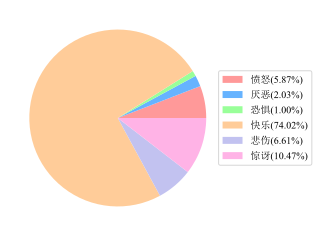
\includegraphics[width=0.5\linewidth]{images/情绪分布.pdf}
	\caption{DailyDialog数据集中情绪分布}
	\label{fig:EmotionPI}
\end{figure}

DailyDialog数据集一共有13118个对话,每轮对话大概有7.8轮且每个句子中大约有29.1个单词。每个对话的轮数以及每个句子中token的个数的箱线图与描述性统计分析如图\ref{fig:sentenceNum}和表\ref{table:sentenceNum}所示。

\begin{table}[!ht]
	\caption{DailyDialog数据集中对话数量与每个句子单词数量的描述性统计分析}
	\label{table:sentenceNum}
	\centering
	\begin{tabularx}{\textwidth}{YYY}
		\toprule
		\textbf{描述性统计分析} & \textbf{每个对话中的轮数} & \textbf{每个句子中token的个数} \\ \midrule
		平均值 & 7.850 & 29.120 \\ 
		最小值 & 2 & 5 \\ 
		25\%分位数 & 4 & 18 \\ 
		50\%分位数 & 7 & 25 \\ 
		75\%分位数 & 10 & 36 \\ 
		最大值 & 35 & 296 \\ \bottomrule
	\end{tabularx}
\end{table}


\begin{table}[!ht]
	\caption{DailyDialog数据集中对话数量与每个句子单词数量的描述性统计分析}
	\label{table:sentenceNum}
	\centering
	\begin{tabularx}{\textwidth}{YYY}
		\toprule
		\textbf{描述性统计分析} & \textbf{每个对话中的轮数} & \textbf{每个句子中token的个数} \\ \midrule
		平均值 & 7.850 & 29.120 \\ 
		最小值 & 2 & 5 \\ 
		25\%分位数 & 4 & 18 \\ 
		50\%分位数 & 7 & 25 \\ 
		75\%分位数 & 10 & 36 \\ 
		最大值 & 35 & 296 \\ \bottomrule
	\end{tabularx}
\end{table}


\subsection{模型的构建}

如前所述,BERT模型对应于[CLS]的输出包含了整个输入句子的语义信息,可以使用这个语义语义信息经过一个分类器得到这句话对应的情感。在对话情感识别中,对话的上下文也包含了一定有助于情感识别的信息,所以在使用BERT编码每个句子之后没有直接利用分类器对句子进行分类,而是利用一个LSTM网络让其获取对话上下文的信息再进行分类。此外,对话的行动也有可能对对话的情感有一定的影响,所以在此次实验中构建了一个多任务的分类器,以促进两个任务的学习。模型的结构如图\ref{fig:MyModel}所示。

\begin{figure}[htb]
	\centering
	\includegraphics[page=14, width=0.75\linewidth]{images/structure.pdf}
	\caption{实验模型主要结构}
	\label{fig:MyModel}
\end{figure}

我进行了多次的消融实验,经过对比分析上述的假设是成立的,且经过预训练的模型BERT对情感识别任务具有强大的作用。

\subsection{实验细节与结果分析}

所有实现均在一台配备RTX 3090显卡(24GB)的Ubuntu计算机上使用PyTorch 2.0完成。由于显存的限制,批量大小均设置为4,学习率设置为$1\mathrm{e}-6$并使用了学习率预热和衰减的方法。

\subsubsection{预训练BERT模型对实验结果的影响}

首先,使用预训练的BERT模型与LSTM组成神经网络,并利用全量更新的方式对模型进行训练。从图\ref{fig:Base}可以看出,对于分类任务而言,由于预训练模型的使用,在第125个batch时就已经收敛到比较高的水平,在验证集中情感分类准确率达到65.03\%。最终在第700个batch达到最高水平,在验证集中情感分类准确率达到66.82\%,且在测试集中的情感分类准确率达到63.10\%。

\begin{figure}[htb]
	\centering
	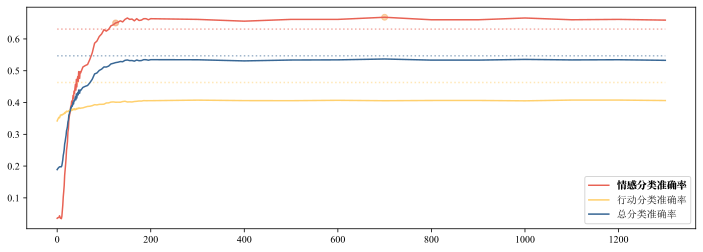
\includegraphics[width=0.75\linewidth]{images/基准.pdf}
	\caption{基准模型实验结果}
	\label{fig:Base}
\end{figure}

在对BERT参数冻结之后,虽然效果相比于全参微调要差(在验证集中情感分类准确率达到64.80\%,且在测试集中的情感分类准确率达到60.59\%),但是由于其不用计算和存储BERT模型参数的梯度,所以计算速度和显存占用量都比全参微调要好,也是一种不错的选择。此外,在对BERT参数重置之后,由于没有使用预训练而直接微调,模型一直无法得到准确的预测。从另一个方面也说明,预训练模型中预训练与微调结合的方法是必不可少的。

\begin{figure}[htb]
	\centering
	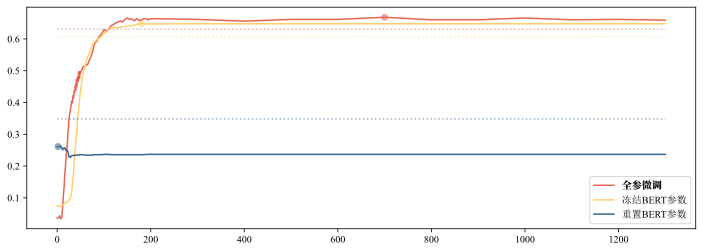
\includegraphics[width=0.75\linewidth]{images/预训练BERT模型.pdf}
	\caption{对预训练编码模型BERT不同的操作实验结果对比}
	\label{fig:PreTraingBert}
\end{figure}

此外,还使用了更大规模的$\text{BERT}_\text{LARGE}$模型进行了比较。由于显存的限制,我冻结了BERT模型的参数,以便进行对比分析。尽管已经对后续神经网络进行了调整,但在投入更多计算资源的情况下,并未观察到性能的显著提升。这表明模型规模的增大并非总能带来更好的效果。对于小型任务,选择规模较小的模型可能会带来更高的效率和更优越的性能,这一点值得注意。

\begin{figure}[htb]
	\centering
	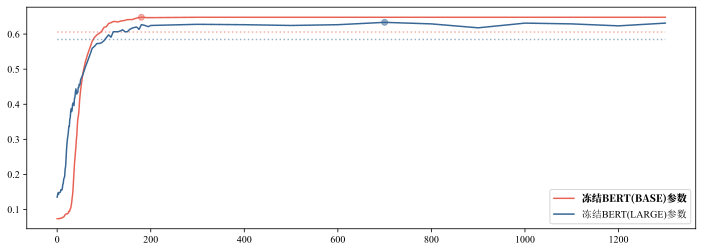
\includegraphics[width=0.75\linewidth]{images/模型大小.pdf}
	\caption{$\text{BERT}_\text{BASE}$模型与$\text{BERT}_\text{LARGE}$模型实验结果之间的对比}
	\label{fig:LargeBert}
\end{figure}

\subsubsection{多任务损失对实验结果的影响}

该实验采用了多任务损失函数,要求BERT和LSTM结构同时学习情感分类和行动分类的信息。当将损失平衡因子$\alpha$设为0时,观察到情感分类准确率下降,表明这种多任务损失对情感分类准确性有所帮助。设置$\alpha$为0.5时,情感分类准确率达到最高值,在测试集中达到了63.33\%。

另外,值得注意的是行动分类的准确率较低。即便将损失平衡因子$\alpha$设为5,准确率仍有所提升但仍然偏低,在测试集上仅为46.73\%。因此,我将多任务损失函数改为仅针对行动进行预测,然而即便如此,行动分类的准确率仍然较低,这表明该模型结构可能不太适用于行动分类任务。

\begin{figure}[htb]
	\centering
	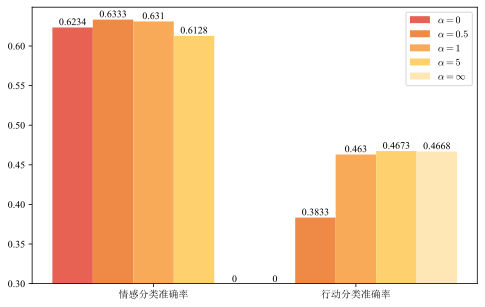
\includegraphics[width=0.55\linewidth]{images/平衡因子.pdf}
	\caption{不同平衡因子$\alpha$之间的情感分类准确率与行动分类准确率的比较}
	\label{fig:alpha}
\end{figure}

值得说明的是,由于将损失平衡因子$\alpha$设置为0.5之后情感分类准确率最高,所以后续的实验均设置$\alpha=0.5$。

\subsubsection{改进模型的结构对实验结果的影响}

\paragraph{BiLSTM网络}

鉴于LSTM网络只能捕获下文信息,我尝试将其改为BiLSTM网络,以便获取上下文信息。然而,我发现准确率提升并不明显,如图\ref{fig:bidirectional2}中黄线所示。这可能是因为使用BiLSTM网络后,参数和输出维度都会翻倍。为了解决这一问题,我将BiLSTM网络中的双层结构改为单层,观察到情感识别准确率有所提升。在验证集上达到了69.91\%,在测试集上达到了65.91\%的准确率。

\begin{figure}[htb]
	\centering
	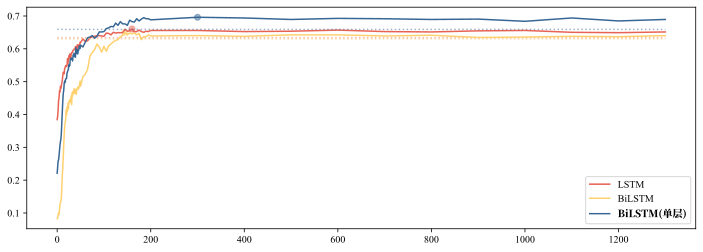
\includegraphics[width=0.75\linewidth]{images/bidirectional.pdf}
	\caption{使用双向LSTM之后的实验结果对比}
	\label{fig:bidirectional2}
\end{figure}

\paragraph{更大的模型结构}

在此次实验中,LSTM的输出维度为1024,BiLSTM的输出维度为$1024\times 2 = 2048$,而情绪和行动分类个数分别为6类和4类,维度的骤降可能不利于模型的泛化,所以我使用了两层的全连接层,其中添加的隐藏层有512个神经元。但是模型的整体表现不佳。

\begin{figure}[htb]
	\centering
	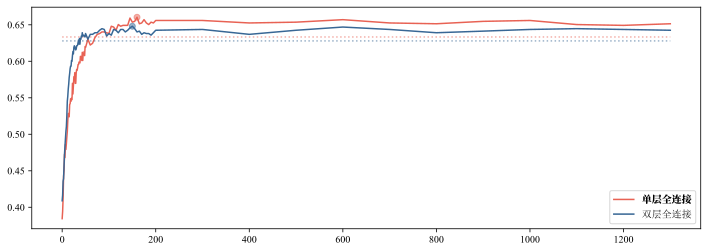
\includegraphics[width=0.75\linewidth]{images/神经网络大小.pdf}
	\caption{使用双层全连接之后实验结果对比}
	\label{fig:size}
\end{figure}

为了进一步增加模型的表达能力,我采用了BiLSTM模型,并适当增加了全连接层的宽度,将隐藏层的输入维度设为4096,输出维度设为1024,并尝试了不同的Dropout参数进行对比。结果显示,采用更大规模的模型在验证集上的效果更佳,但仍然存在过拟合问题。

\begin{figure}[htb]
	\centering
	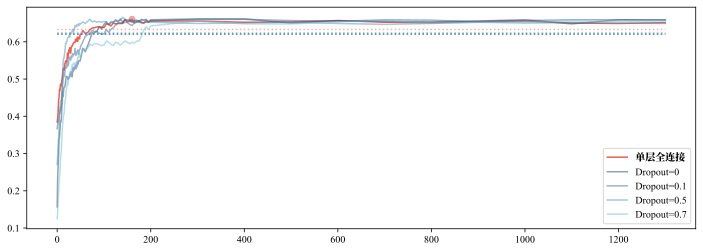
\includegraphics[width=0.75\linewidth]{images/Dropout.pdf}
	\caption{使用Dropout技术之后的实验结果对比}
	\label{fig:Dropout2}
\end{figure}

\paragraph{RNN和GRU}

正如之前提到的,除了LSTM网络外,循环神经网络还包括RNN网络和GRU网络等变种。我对比了将LSTM网络替换为其他类型的循环神经网络。结果显示,采用RNN网络的准确率比使用LSTM网络和GRU网络更高。在验证集上,准确率达到了66.59\%,在测试集上也有64.54\%的准确率。

\begin{figure}[htb]
	\centering
	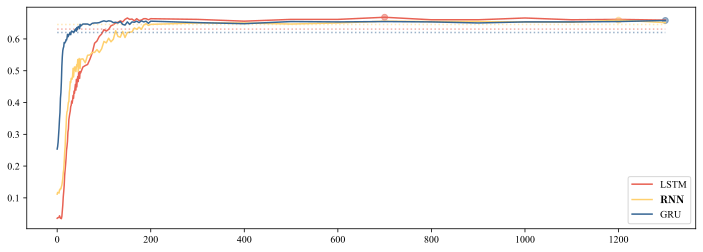
\includegraphics[width=0.75\linewidth]{images/循环结构.pdf}
	\caption{不同的循环神经网络实验结果的比较}
	\label{fig:structure}
\end{figure}

\subsubsection{不使用上下文信息对实验结果的影响}

由于预训练编码模型BERT经过大量数据进行无监督预训练,并在多种下游任务中进行微调,其编码能力很强大,所以我也尝试不使用循环神经网络融合上下文信息,直接将BERT的输出传递给前连接层,发现获得比较好的效果。在平衡因子$\alpha$设为0.5时,$\text{BERT}_\text{BASE}$模型在测试集中的情感分类准确率达到了70.99\%,不经过微调的$\text{BERT}_\text{LARGE}$模型的准确率也有70.16\%。此外,从图\ref{fig:context}中可以看出,$\text{BERT}_\text{BASE}$模型刚开始训练就已经达到很高的准确率。

\begin{figure}[htb]
	\centering
	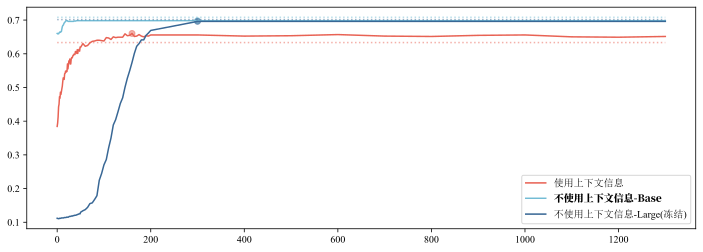
\includegraphics[width=0.75\linewidth]{images/对话上下文.pdf}
	\caption{是否使用循环结构的实验结果对比}
	\label{fig:context}
\end{figure}

从\ref{fig:context}图中可以看出,使用LSTM提取上下文信息可能会削弱预训练编码模型BERT的表达能力,反而会让分类任务性能有所下降。另外,当平衡因子$\alpha$设为1时,我们获得了本次实验最佳且最平衡的成绩\footnote{为了获得最均衡的成绩,保存的模型是总分类准确率最好的模型而不是情感分类准确率最好的模型。}。在测试集中,情感分类准确率达到了70.99\%,行动分类准确率达到了71.80\%,总体分类准确率达到了71.40\%。

\begin{figure}[htb]
	\centering
	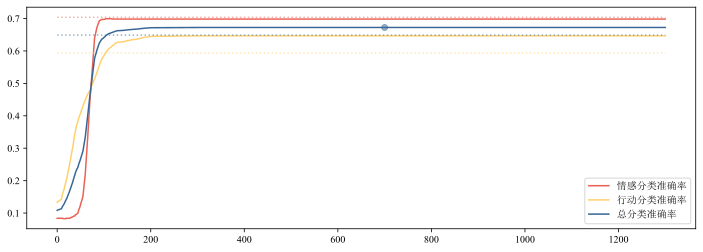
\includegraphics[width=0.75\linewidth]{images/TheBest.pdf}
	\caption{此次实验中最好的模型实验结果}
	\label{fig:theBest}
\end{figure}

\subsubsection{实验结果汇总与分析}

除了上述所描述的实验结果,本实验还针对其他参数做了许多消融实验,实验结果如表\ref{table:result}所示。其中,下划线为影响某个因素中的最好结果,加粗为整个实验中的最好结果。

\begin{landscape}
	\zihao{6}
	\begin{table}[!ht]
	\centering
	\zihao{-5}
	\caption{实验结果汇总}
	\label{table:result}
	\begin{tabular}{ccccccccc}
		\toprule
		\textbf{影响因素} & \textbf{BERT} & \textbf{循环结构} & \textbf{线性层数量} & \textbf{Dropout} & \textbf{平衡因子$\alpha$} & \textbf{ALLACC} & \textbf{EmotionACC} & \textbf{ActACC} \\ \midrule
		\multirowcell{4}{预训练BERT模型} & 全参 & LSTM & 单层 & 0 & 1 & \underline{0.5470} & \underline{0.6310} & \underline{0.4630} \\ 
		~ & 冻结 & LSTM & 单层 & 0 & 1 & 0.5191 & 0.6059 & 0.4323 \\ 
		~ & 重置 & LSTM & 单层 & 0 & 1 & 0.3026 & 0.3485 & 0.2567 \\ 
		~ & Large+冻结 & LSTM(2048) & 单层 & 0 & 1 & 0.5050 & 0.5847 & 0.4253 \\ \midrule
		\multirowcell{4}{平衡因子$\alpha$} & 全参 & LSTM & 单层 & 0 & 0 & - & 0.6234 & - \\ 
		~ & 全参 & LSTM & 单层 & 0 & 0.5 & 0.5083 & \underline{0.6333} & 0.3833 \\ 
		~ & 全参 & LSTM & 单层 & 0 & 5 & 0.5400 & 0.6128 & \underline{0.4673} \\ 
		~ & 全参 & LSTM & 单层 & 0 & $\infty$ & - & - & 0.4668 \\ \midrule
		\multirowcell{4}{bidirectional} & 全参 & BiLSTM & 单层 & 0 & 0.5 & 0.5310 & 0.6302 & 0.4318 \\ 
		~ & 全参 & BiLSTM & 单层 & 0 & 1 & 0.5193 & 0.6143 & 0.4243 \\ 
		~ & 全参 & BiLSTM(单层) & 单层 & 0 & 0.5 & 0.5539 & \underline{0.6591} & 0.4488 \\ 
		~ & 全参 & BiLSTM(单层) & 单层 & 0 & 1 & 0.5882 & 0.6538 & \underline{0.5226} \\ \midrule
		\multirowcell{5}{线性层数量\\与Dropout} & 全参 & LSTM & 双层(1024, 512) & 0 & 0.5 & 0.5392 & 0.6279 & 0.4506 \\ 
		~ & 全参 & Bi-LSTM(2048) & 双层(4096, 1024) & 0 & 0.5 & 0.5286 & 0.6203 & 0.4368 \\ 
		~ & 全参 & Bi-LSTM(2048) & 双层(4096, 1024) & 0.1 & 0.5 & 0.5201 & 0.6211 & 0.4191 \\ 
		~ & 全参 & Bi-LSTM(2048) & 双层(4096, 1024) & 0.5 & 0.5 & 0.5271 & 0.6226 & 0.4315 \\ 
		~ & 全参 & Bi-LSTM(2048) & 双层(4096, 1024) & 0.7 & 0.5 & 0.5290 & 0.6249 & 0.4331 \\ \midrule
		\multirowcell{2}{循环结构} & 全参 & RNN & 单层 & 0 & 1 & \underline{0.5863} & \underline{0.6454} & 0.5272 \\ 
		~ & 全参 & GRU & 单层 & 0 & 1 & 0.5220 & 0.6203 & 0.4237 \\ \midrule
		\multirowcell{3}{对话上下文} & 全参 & None & 单层 & 0 & 0.5 & 0.6990 & \underline{\textbf{0.7099}} & 0.6881 \\ 
		~ & 全参 & None & 单层 & 0 & 1 & \underline{\textbf{0.7140}} & \underline{\textbf{0.7099}} & \underline{\textbf{0.7180}} \\ 
		~ & Large+冻结 & None & 单层 & 0 & 0.5 & 0.5801 & 0.7016 & 0.4585 \\ \bottomrule
	\end{tabular}
\end{table}
\end{landscape}


从上述实验可以看出,预训练编码模型BERT具有强大的表达能力,在经过较少的训练就能够达到很好的性能。在使用预训练编码模型时应该注意:

\begin{itemize}
	\item \textbf{分类器的复杂度平衡:}针对简单的分类任务时,选择的分类器应该匹配任务的复杂度。过于复杂的分类器可能会削弱预训练模型原有的表达能力。因此,在设计分类器时需要在精度和模型复杂度之间取得平衡。
	\item \textbf{任务大小与预训练模型的选择:}根据任务的规模和复杂程度选择适当大小的预训练编码模型是至关重要的。对于小型任务,选择相对较小的预训练模型既能提高模型的性能,又能提升模型运行的效率。这样做还有助于减少资源需求,加快训练和推理速度。
	\item \textbf{迁移学习策略:}在使用预训练编码模型时,需要考虑迁移学习的策略。有时候,仅冻结预训练模型的底层,只微调顶层,或者通过逐步解冻层来逐渐微调模型,都是有效的迁移学习策略。选择适当的策略有助于平衡模型的泛化能力和训练速度。
	\item \textbf{领域特定的微调:}某些情况下,预训练编码模型的泛化能力可能不足以完全适应特定领域的任务。在这种情况下,需要考虑在预训练模型上进行领域特定的微调,以提高模型在特定领域的性能。
	\item \textbf{超参数调整:}不同的任务和数据集可能需要不同的超参数设置。对于使用预训练编码模型的任务,经常需要对学习率、批量大小、优化器等超参数进行调整,以获得更好的性能。
\end{itemize}


















































































